%-------------------------------------------------------------------------------

% This file is part of code_saturne, a general-purpose CFD tool.
%
% Copyright (C) 1998-2022 EDF S.A.
%
% This program is free software; you can redistribute it and/or modify it under
% the terms of the GNU General Public License as published by the Free Software
% Foundation; either version 2 of the License, or (at your option) any later
% version.
%
% This program is distributed in the hope that it will be useful, but WITHOUT
% ANY WARRANTY; without even the implied warranty of MERCHANTABILITY or FITNESS
% FOR A PARTICULAR PURPOSE.  See the GNU General Public License for more
% details.
%
% You should have received a copy of the GNU General Public License along with
% this program; if not, write to the Free Software Foundation, Inc., 51 Franklin
% Street, Fifth Floor, Boston, MA 02110-1301, USA.

%-------------------------------------------------------------------------------

%===============================================
\section{ Gas combustion}
%===============================================

Flames with gaseous fuels can be categorized in premix, diffusion or
partial-premix.

%=======================================
\subsection{Premix: Eddy Break Up}
%=======================================

The original Spalding model \cite{Spalding:1971a} was written for a situation where the whole
boiler is filled with the same mixture (only one inlet); the motto of which is
\textit{"If it mixes, it burns"}. If the chemistry is fast vs. mixing, fluid
particles are made of fresh gases or of burned ones. This situation is described
by a progress variable (valued 0 in fresh gases and 1 in burnt ones) with a
source term: the reaction one. The mixture of totally fresh or totally burnt
gases, called intermittency, leads to a maximal variance of the progress
variable determined by the mean value of the progress variable.

\begin{equation}
C"^{2}_{\mbox{\footnotesize max}} = (C_{\mbox{\footnotesize moy}} -C_{\mbox{\footnotesize min}}).(C_{\mbox{\footnotesize max}}-C_{\mbox{\footnotesize moy}}) = C_{\mbox{\footnotesize moy}} . (1-C_{\mbox{\footnotesize moy}})
\end{equation}

The mixing of fresh and burnt gases is the dissipation of this variance and it
induces the conversion of fresh gases in burnt ones. So the source term for the
(mean) progress variable is the dissipation of its (algebraic) variance. Be
careful: in \CS~ the variable chosen to describe the reaction is the mass
fraction of fresh gases (valued 1 in fresh and 0 in burnt), so:

\begin{equation}
S(Y_{\mbox{\footnotesize fg}}) = - C_{\mbox{\small ebu}}~\frac{\epsilon}{k} \displaystyle\left[~\rho ~Y_{\mbox{\footnotesize fg}} \left(1-Y_{\mbox{\footnotesize fg}}\right)\right]
\end{equation}

Where $C_{\mbox{\small ebu}}$ is a constant, supposedly "universal", fitted
around $1.6$ (only advanced users may adjust this value).\\
Some improvements have been proposed, and largely used, for situations with
mixture fraction gradient (staggering of reactant(s)) but are not theorically
funded. The simplest extension is available (options 2 and 3 ) in \CS~ with one
extra equation solved for $f$ the mean of mixture fraction: the corresponding
hypothesis is \textit{"no variance for mixture fraction"} ... a little bit
surprising in an EBU context (maximal variance for progress variable). The
choice of the fresh gas mass fraction appears now to be quite relevant : the
computation of species mass fraction can be done, with respect to the mean
mixture fraction, both in fresh (the mass fraction of which is
$Y_{\mbox{\footnotesize fg}}$) where species mass fraction are obvious and burnt
gases (the mass fraction of which is $(1-Y_{\mbox{\footnotesize fg}})$) among
which species mass fraction come from a complete reaction assumption (as
introduced hereafter for diffusion flame).

\begin{eqnarray}
\displaystyle Y_{\mbox{\footnotesize fuel}} &=&     Y_{\mbox{\footnotesize fg}} . f + (1-Y_{\mbox{\footnotesize fg}}) . \max \left(0 ~;~\frac{f- f_{\mbox{\footnotesize s}}}{1-f_{\mbox{\footnotesize s}}}\right)       \nonumber       \\
\displaystyle Y_{\mbox{\footnotesize Ox}}   &=&     Y_{\mbox{\footnotesize fg}} . (1-f) + (1-Y_{\mbox{\footnotesize fg}}) . \max \left(   0 ~;~\frac{f_{\mbox{\footnotesize s}}-f}{f_{\mbox{\footnotesize s}}}\right)   \label{Eq_001a} \\
\displaystyle Y_{\mbox{\footnotesize prod}} &=& (1-Y_{\mbox{\footnotesize fg}}) . \left( \frac{f}{f_{\mbox{\footnotesize s}}}~;~\frac{1-f}{1-f_{\mbox{\footnotesize s}}} \right)                         \nonumber
\end{eqnarray}
Where $f_{\mbox{s}}$ is the \underline{\bf s}toechiometric mixture
\underline{\bf f}raction.

In adiabatic conditions the specific enthalpy of gases ({\small in every
  combustion model the considered enthalpy contains formation one and heat
  content, but no terms for velocity or pressure}) is directly related to the
mixture fraction ({\small as long as the inlet temperature for air and fuel is
  known}). When heat losses, like radiation, are taken into account, an equation
has to be solved for the mean enthalpy ({\small such an equation is needed so
  when some inlets have different temperatures -partial preheat- enthalpy is
  then used as an extra passive scalar}). In industrial processes, the aim is
often to transfer the heat from burnt gases to the wall; even for heat loss the
wall temperature is near to the fresh gases temperature and the main heat flux
takes place between burnt gases and wall. So, in \CS, the specific enthalpy of
the fresh gases is supposed to be related to mixture fraction and the specific
enthalpy of burnt gases is locally computed to reach the mean specific
enthalpy. By this way every heat loss removed from the mean enthalpy is charged
to the hottest gases.

\begin{equation}
\tilde h = Y_{\mbox{\footnotesize fg}}~.~h_{\mbox{\footnotesize fg}}( \tilde f) + (1-Y_{\mbox{\footnotesize fg}})~.~h_{\mbox{\footnotesize bg}} \quad \Leftrightarrow \quad
                  h_{\mbox{\footnotesize bg}}  = \frac{ \tilde h-Y_{\mbox{\footnotesize fg}}~.~h_{\mbox{\footnotesize fg}}(\tilde f) }{ 1-Y_{\mbox{\footnotesize fg}} }
\end{equation}
%
where $\tilde f$ is here the local mean of the mixture fraction or a constant value ({\small in the regular EBU model}).

%================================================
\subsection{Diffusion: PDF with 3 points chemistry}
%================================================

In diffusion model, the combustion is assumed to be limited only by mixing
(between air and fuel), so the reaction is assumed to reach instantaneously its
equilibrium state and the temperature and concentrations can be computed for
every value of the mixture fraction. In \CS~ the implemented version uses an
extra hypothesis: the reaction is complete; so if the mixture is
stoechiometric, the burnt gases contains only final products (none unburnt like
CO, except definition of product including a specified ratio of CO).  As a
consequence, every concentration is a piecewise linear function of the mixture
fraction (subroutines: \fort{d3pphy, d3pint, cpcym, fucym}).

\begin{eqnarray}
\displaystyle 0         \le f \le f_{\mbox{\footnotesize s}} &;& Y_{i}(f) = Y_{\mbox{\footnotesize air}} + \quad \frac{f}{f_{\mbox{\footnotesize s}}} ~~ (Y_{\mbox{s}}-Y_{\mbox{\footnotesize air}})  \\
\displaystyle f_{\mbox{\footnotesize s}} \le f \le 1         &;& Y_{i}(f) = Y_{\mbox{\footnotesize s}}~~ + \frac{f-f_{\mbox{\footnotesize s}}}{1-f_{\mbox{\footnotesize s}}}~(Y_{\mbox{\footnotesize fuel}}-Y_{\mbox{\footnotesize s}})
\end{eqnarray}

%========================================
\begin{figure}[!htbp]
\centerline{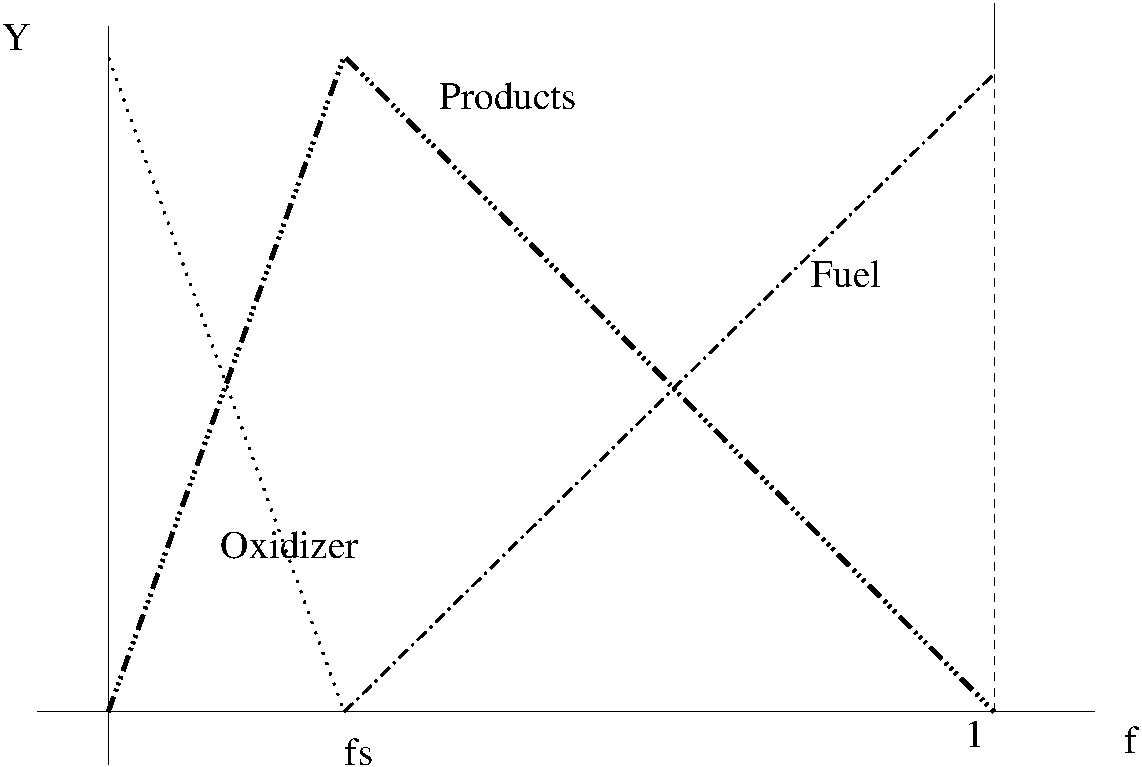
\includegraphics[width=0.8\textwidth]{Yf}}
\caption{Mass fraction of global species are piecewise linear with mixture fraction.}
\end{figure}
%========================================

Where $f_{\mbox{\footnotesize s}}$ is the stoechiometric mixture fraction, $Y_s$
the concentrations in products of the complete reaction of a stoechiometric
mixture (in such products, the chemical reaction is no more possible :
inert). Beware to distinguish $Y_{\mbox{\footnotesize fuel}}$ mass fraction of a
species (depending on f) and $Y_{\mbox{\footnotesize fuel}}$ mass fraction of
species in
the inlet condition for the fuel stream ($Y_{i,\mbox{\footnotesize fuel}} = Y_{i}(1) \quad Y_{i,\mbox{\footnotesize air}} = Y_{i}(0)$). \\
The diffusion model uses two equations for the mixture fraction and its
variance. Both of them having no reaction term. The mean and the variance of the
mixture fraction are used to fit parameter of a Probability Density Function,
with a presumed form, for the mixture fraction. In \CS~ the shape proposed by
\cite{Borghi:1978a} with a rectangle and Dirac's peak is used (subroutines \fort{copdf,
  cppdf, fupdf}).

%========================================
\begin{figure}[!htbp]
\centerline{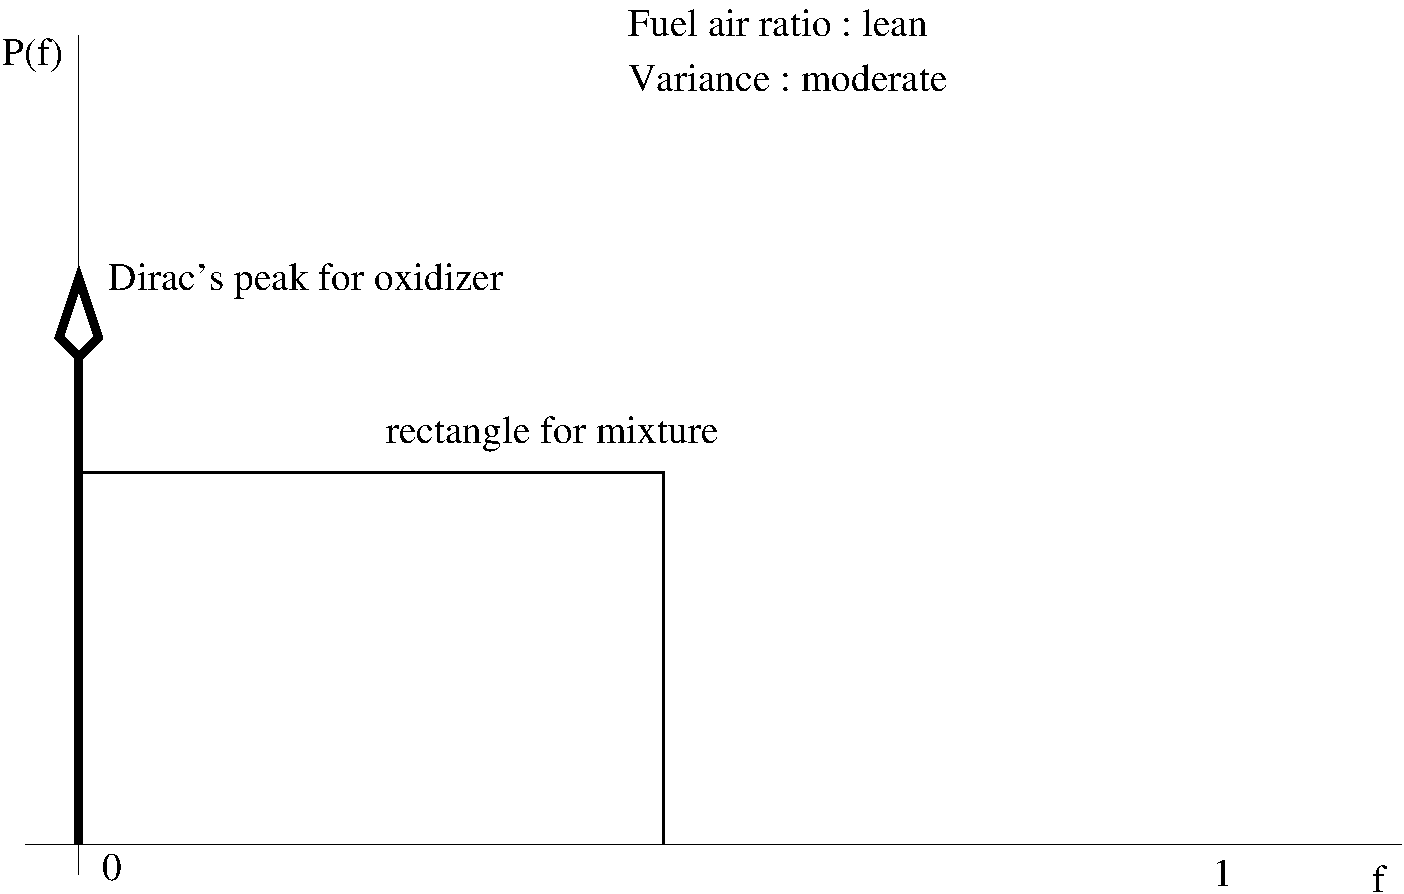
\includegraphics[width=0.8\textwidth]{Pf}}
\centerline{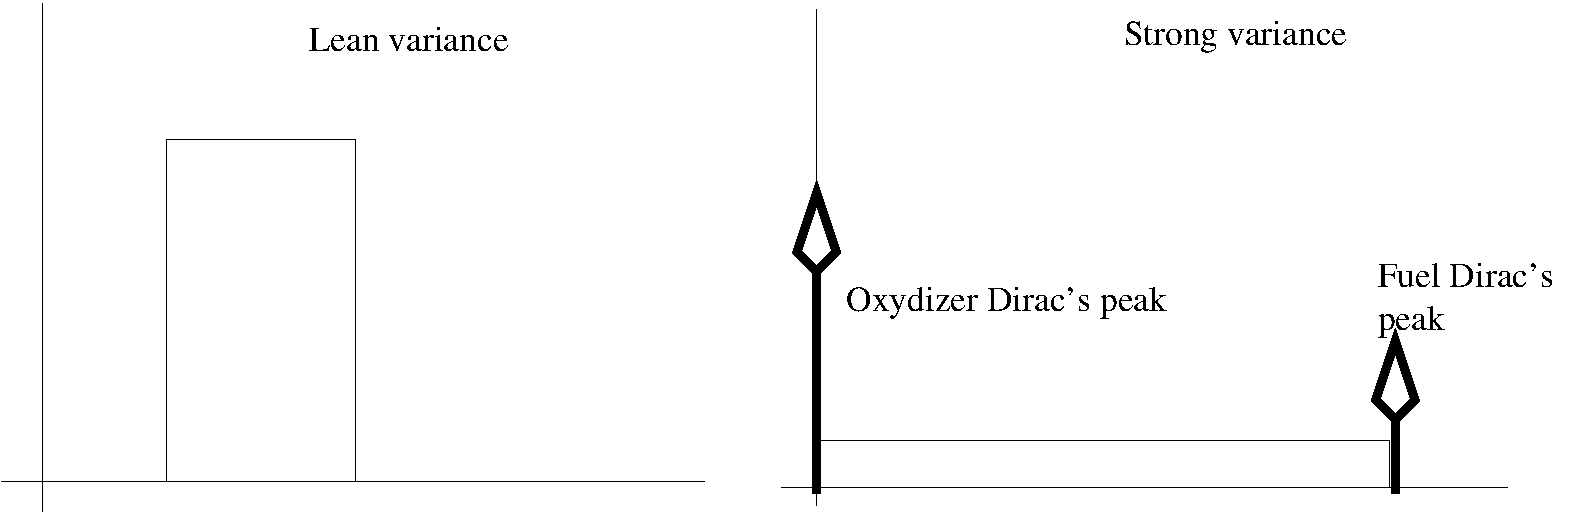
\includegraphics[width=0.8\textwidth]{Pf2}}
\caption{Examples of presumed PDF: cheapest form.}
\end{figure}
%========================================

The determination of the mean concentration is done by integrating the local
concentration weighted by the probability density function. As a matter of fact,
integrating the product of a piecewise linear function by a constant (height of
the rectangle) is a very simple exercise: analytic
solution is available (the original formulation \cite{Borghi:1978a} which uses $\beta$ function was much more computationaly expensive).\\
In adiabatic condition, the specific enthalpy of the mixture is a linear
function of the mixture fraction (the enthalpy is not modified by the
reaction). As for premixed combustion, the following assumption is done
\textit{"the hotter the gases, the worse the heat losses"}, so the enthalpy of
pure oxidizer and fuel are supposed to be not modified in permeatic conditions,
the enthalpy of products $h_{\mbox{\footnotesize s}}$ (at the stoechiometric
mixture fraction) is an unknown or auxiliary variable. The enthalpy of the
mixture is supposed linear piecewise with $f$ (like concentrations but with an
unkwnon at $f_{\mbox{\footnotesize s}}$) and the resulting mean enthalpy
(weighted by PDF) is linear in $h_{\mbox{\footnotesize s}}$.  Fitting with the
equation for the mean enthalpy (which takes in account radiation and other heat
fluxes), $h_{\mbox{\footnotesize s}}$ is determined and, consequently the
temperature at fs and the mean temperature can be computed.

%========================================
\begin{figure}[!htbp]
\centerline{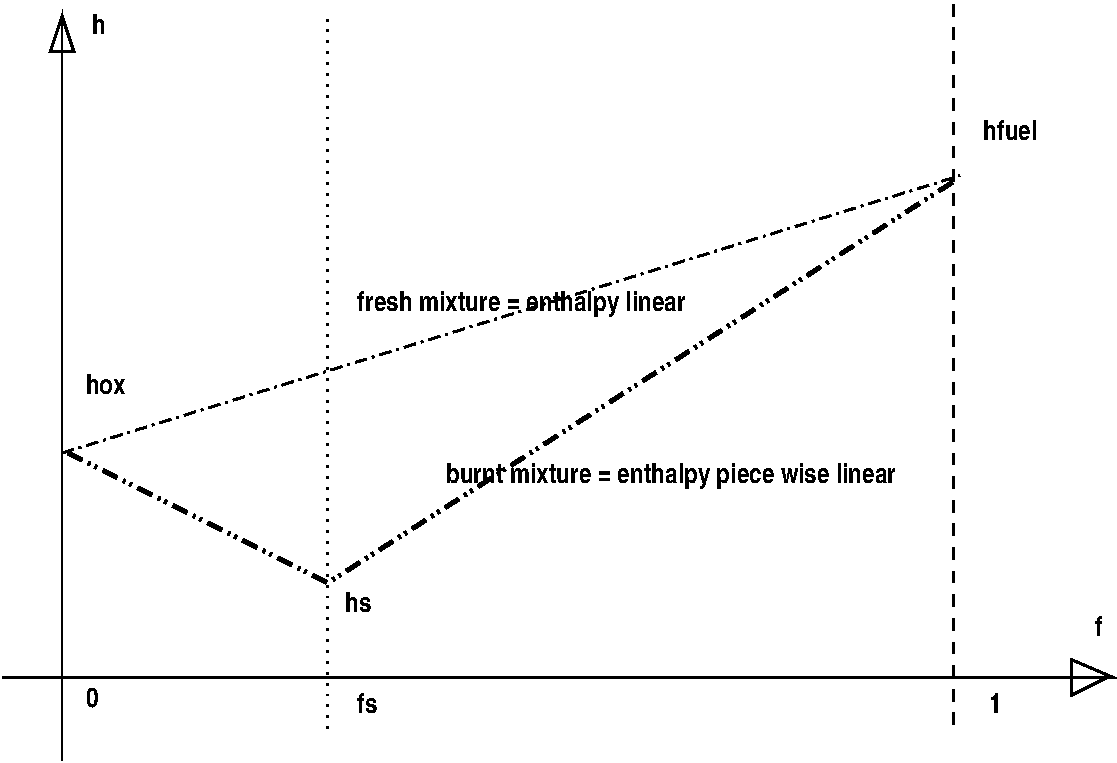
\includegraphics[width=0.8\textwidth]{hf}}
\caption{Enthalpy of products is determined to take in account the heat losses.}
\end{figure}
%========================================
As an example of the capabilities of the simple pdf used in \CS, computations
for the determination of the value of this auxiliary variable are detailed
hereafter.

\begin{eqnarray}
\displaystyle 0  \le f \le f_{\mbox{s}} &;& h_{\ell} = h_{\mbox{\small Ox}} + \left(~h_{\mbox{\footnotesize s}} - h_{\mbox{\small Ox}}~\right)~\frac{f}{f_{\mbox{\footnotesize s}}} \nonumber\\
\displaystyle f_{\mbox{\footnotesize s}} \le f \le 1  &;& h_{\mbox{\footnotesize s}} = \frac{f_{\mbox{\footnotesize s}}.~h_{\mbox{\footnotesize fuel}} - h_{\mbox{\footnotesize s}} }{f_{\mbox{\footnotesize s}}-1} + \left( h_{\mbox{\footnotesize s}}-h_{\mbox{\footnotesize fuel}} \right)~\frac{f}{f_{\mbox{\footnotesize s}}-1}
\end{eqnarray}\vspace{-0.22in}
\begin{eqnarray}
\displaystyle\int_{0}^1 h(f) . P(f) df &=& D_0.h_{\mbox{\small Ox}} + D_1.h_{\mbox{\footnotesize fuel}} \qquad\qquad\qquad\nonumber \\
                          &+& \int_{\displaystyle f_{1,\ell} = \min(f_1,f_{\mbox{\footnotesize s}})}^{\displaystyle f_{2,\ell} = \min(f_{\mbox{\footnotesize s}},f_2)} h_{\ell}(f) . H . df \qquad\qquad\qquad\qquad\qquad\qquad\label{Eqs_00B} \\
\displaystyle                          &+& \int_{\textstyle f_{1,r} = \max(f_1,f_{\mbox{\footnotesize s}})}^{\textstyle f_{2,r} = \max(f_{\mbox{\footnotesize s}},f_2)} h_{r}(f) . H . df \qquad\qquad\qquad\qquad\nonumber
%---------------
\end{eqnarray}
\vspace{-0.22in}
\begin{eqnarray}
%---------------
\int_{0}^1 h(f) . P(f) df &=& D_0.h_{\mbox{\small Ox}} + D_1.h_{\mbox{\footnotesize fuel}} \qquad \qquad\nonumber \\
                          &+& H. h_{\mbox{\small Ox}} . (f_{2,\ell}-f_{1,\ell})
                           +  H.(h_{\mbox{\footnotesize s}}-h_{\mbox{\footnotesize air}})~
\left\{ \frac{f_{2,\ell}^2-f_{1,\ell}^2}{2~f_{\mbox{\footnotesize s}}} \right\}\label{Eqs_00C} \\
                          &+& H . \frac{f_{\mbox{\footnotesize s}}.h_{\mbox{\footnotesize fuel}}-h_{\mbox{\footnotesize s}}}{f_{\mbox{\footnotesize s}}-1} . (f_{2,r}-f_{1,r}) + H. (h_{\mbox{\footnotesize s}}-h_{\mbox{\footnotesize fuel}})
\displaystyle \left\{ \displaystyle \frac{f_{2,r}^2-f_{1,r}^2}{2~(f_{\mbox{\footnotesize s}}-1)} \right\}\nonumber
%---------------
\end{eqnarray}
\vspace{-0.25in}
\begin{eqnarray}
%---------------
\int_{0}^1 h(f) . P(f) df &=& D_0.h_{\mbox{\small Ox}} + D_1.h_{\mbox{\footnotesize fuel}} \qquad\qquad\nonumber \\
                          &+& \underbrace{H ~ h_{\mbox{\small Ox}} ~ (f_{2,\ell}-f_{1,\ell})
                           -  H ~ h_{\mbox{\small Ox}}
\displaystyle{     ~\frac{(f_{2,\ell}^2-f_{1,\ell}^2)}{2~f_{\mbox{\footnotesize s}}} } }_{\displaystyle H_{\small Ox}~;~\mbox{2 terms}}\qquad\qquad\nonumber \\
                          &+& \underbrace{H ~ ~h_{\mbox{\footnotesize fuel}} ~\frac{ f_{\mbox{\footnotesize s}}
                                              ~(f_{2,r}-f_{1,r}) }{ (f_{\mbox{\footnotesize s}}-1) }
                            - H ~ h_{\mbox{\footnotesize fuel}} ~ \displaystyle{\frac{(f_{2,r}^2-f_{1,r}^2)}{2.(f_{\mbox{\footnotesize s}}-1)} } }_{   \displaystyle H_{\mbox{\small fuel}}~;~\mbox{2 terms} }\qquad\qquad \\
                          &+& \underbrace{ H . h_{\mbox{\footnotesize s}} ~
\displaystyle \left\{ \frac{(f_{2,\ell}^2-f_{1,\ell}^2)}{2~f_{\mbox{\footnotesize s}}}
                -\frac{(f_{2,r}-f_{1,r})          }{(f_{\mbox{\footnotesize s}}-1)}
                +\frac{(f_{2,r}^2-f_{1,r}^2)}{2~(f_{\mbox{\footnotesize s}}-1)} \right\} }_{\displaystyle H^{*}~;~\mbox{last terms}} \qquad\qquad\nonumber
%---------------
\end{eqnarray}

With $h_{\ell}$ enthalpy on the \underline{\bf l}ean side of
$f_{\mbox{\footnotesize s}}$, $h_{r}$ enthalpy on the \underline{\bf r}ich side; $D_0$ the Dirac's peak in pure air, $D_1$ Dirac's peak in
pure fuel, $f_1$ begin of rectangle, $f_2$ end of rectangle, $H$ heigth of rectangle.

This expression for enthalpy includes a last term linear in
$h_{\mbox{\footnotesize s}}$ , identification with the transported enthalpy
(solved with source term for radiation and so on) allows to determine its value:

\begin{eqnarray}
\int_{0}^1 h(f) . P(f) df =\tilde{h} \quad  \Leftrightarrow &&
                    h_{s} =\frac{\tilde{h}- [ D_0.h_{\mbox{\small air}} + D_1.h_{\mbox{\small fuel}}+\{ H_{\mbox{\small Ox}} + H_{\mbox{\small fuel}}\} ]}{H^{*}}
\end{eqnarray}

%================================================
\subsection{Partial premix: Libby Williams models}
%================================================

\CS~ has been the test-bench for some versions of Libby-Williams model \cite{Libby:2000a},
like for the models implemented and then incremented by \cite{Ribert:2004a} and \cite{Robin:2005a}.

The Libby \& Williams model have been developed to address the description of
the combustor can of gas turbine in regime allowing a reduction of NOx
production using (sometimes very) lean premix. By this way, the combustion
occurs at moderate temperatures avoiding the hot spots which are favourable to
thermal NOx production. Because of the moderate temperatures, the chemistry is
no more so fast and the stability is questionnable. To ensure it a diffusion
flame called pilot takes place in the center of the combustor. So, if the main
flow is premixed, both pure fuel and pure oxidiser are introduced in the
combsutor leading to continuous variation of the equivalence ratio (always the
mixture fraction).This situation is clearly out of the range of both EBU and PDF
models, moreover the limitation by the chemistry is needed (for stability studies).

Originally, Libby \& Williams proposed a presumed PDF made of two Dirac's peaks,
Ribert showed that this PDF could be determined with only the mean and the
variance of the mixture fraction and a reactive variable (by now, the mass
fraction of fuel is used). Then some undeterminations seem awkward and Robin
\emph{et al.} propose a four Dirac's peaks PDF whose parameters are determined with the
same variables and the solved ({\small transported}) covariance (of the reactive
variable and the mixture fraction) as an extra solved field. With the condition
corresponding to every Dirac's peak, a global chemistry description is used (the
source term for every variables is a weighting of the reaction fluxes).

With two peaks distribution, the two-variable PDF is restricted to one line,
crossing the mean state and the slope of which is the ratio of
variances (choice of the sign is user free, ... but relevant: expertise is needed). The correlation between variables is unity.
On this line the distribution is supposed to obey a modified Curl model \cite{Curl:1963a}.

%========================================
\begin{figure}[!htpb]
\centerline{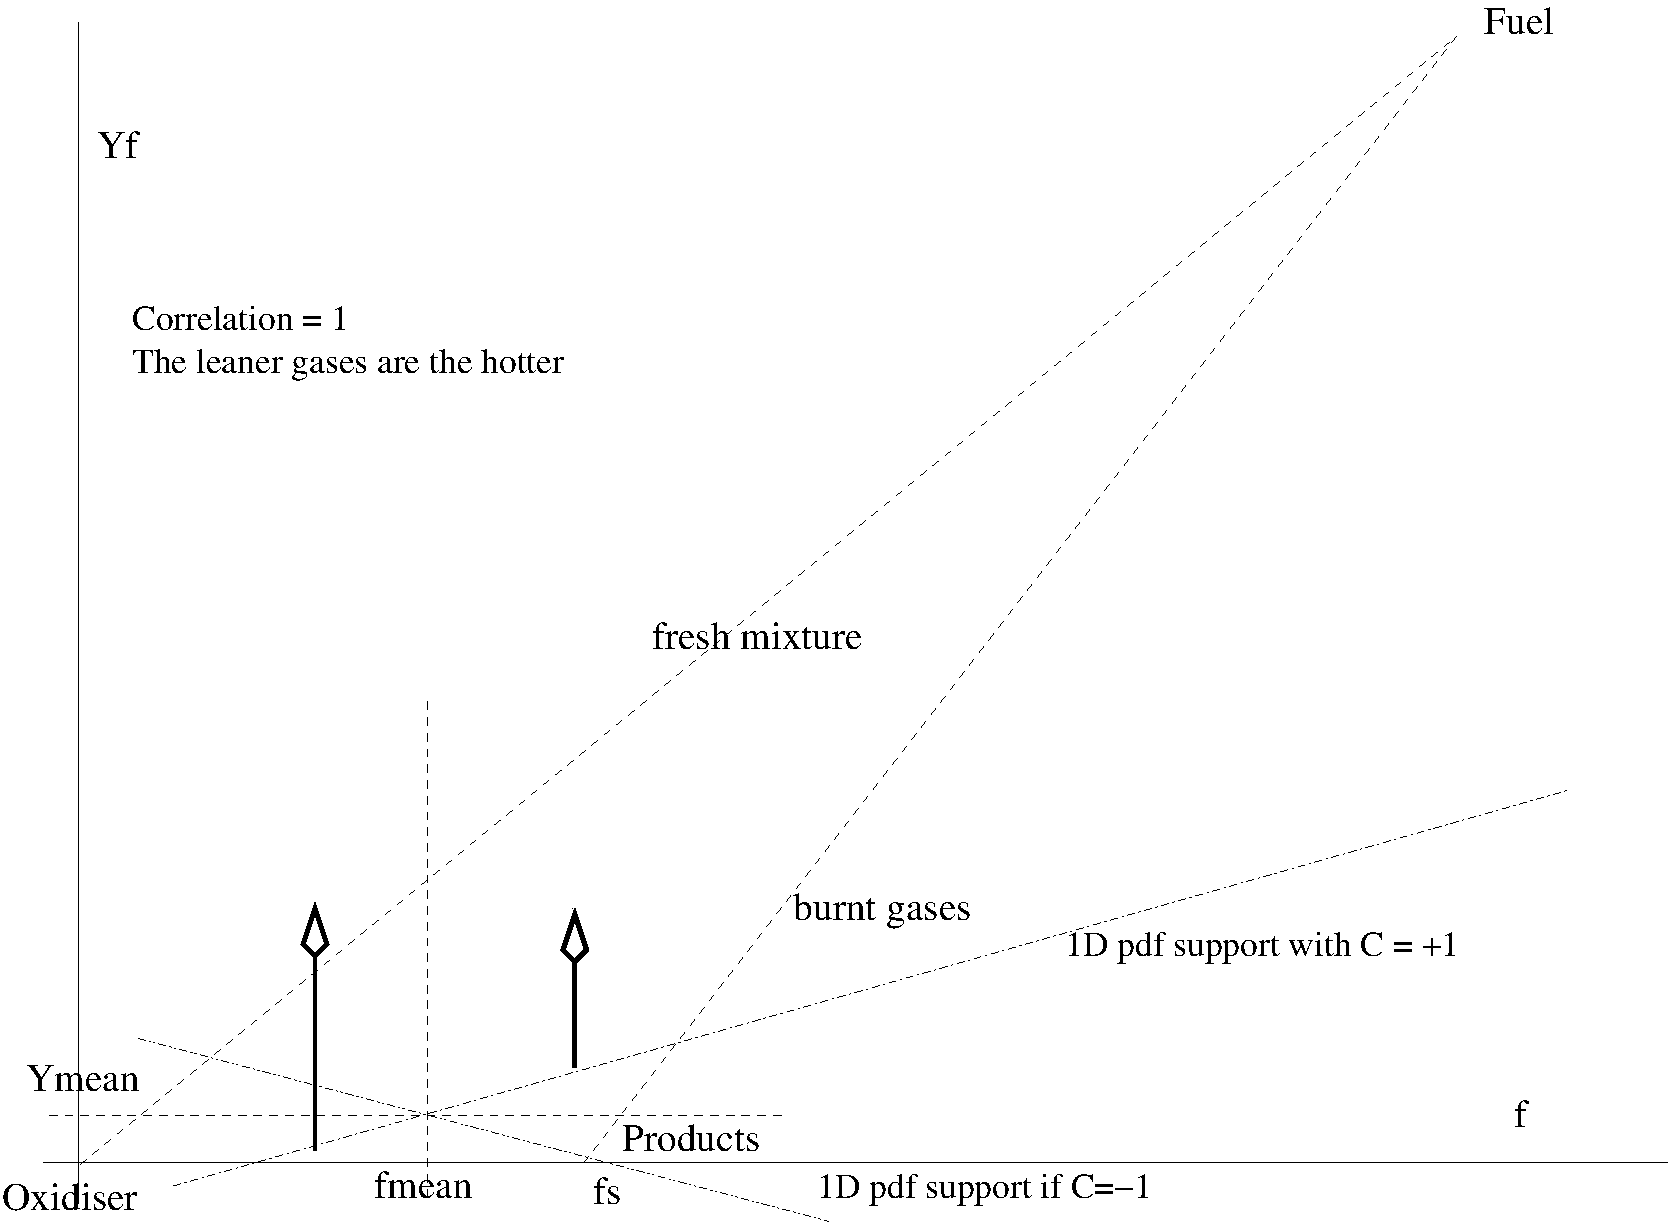
\includegraphics[width= 0.8\textwidth]{LW2}}
\caption{PDF recommended by Libby \& Williams: still undetermined.}
\end{figure}
%========================================
With three or four peaks distribution, the whole concentration space is
available and the determination of the covariance allows evolution of the
correlation (with $f$ and $Yf$, it has been shown that the correlation is positive
in mixing layer and can become negative across the flame: the
particle nearer of stoechiometry being able to burn -then destroy Yf- faster than the particles in poor regime). \\
%========================================
\begin{figure}[!htpb]
\centerline{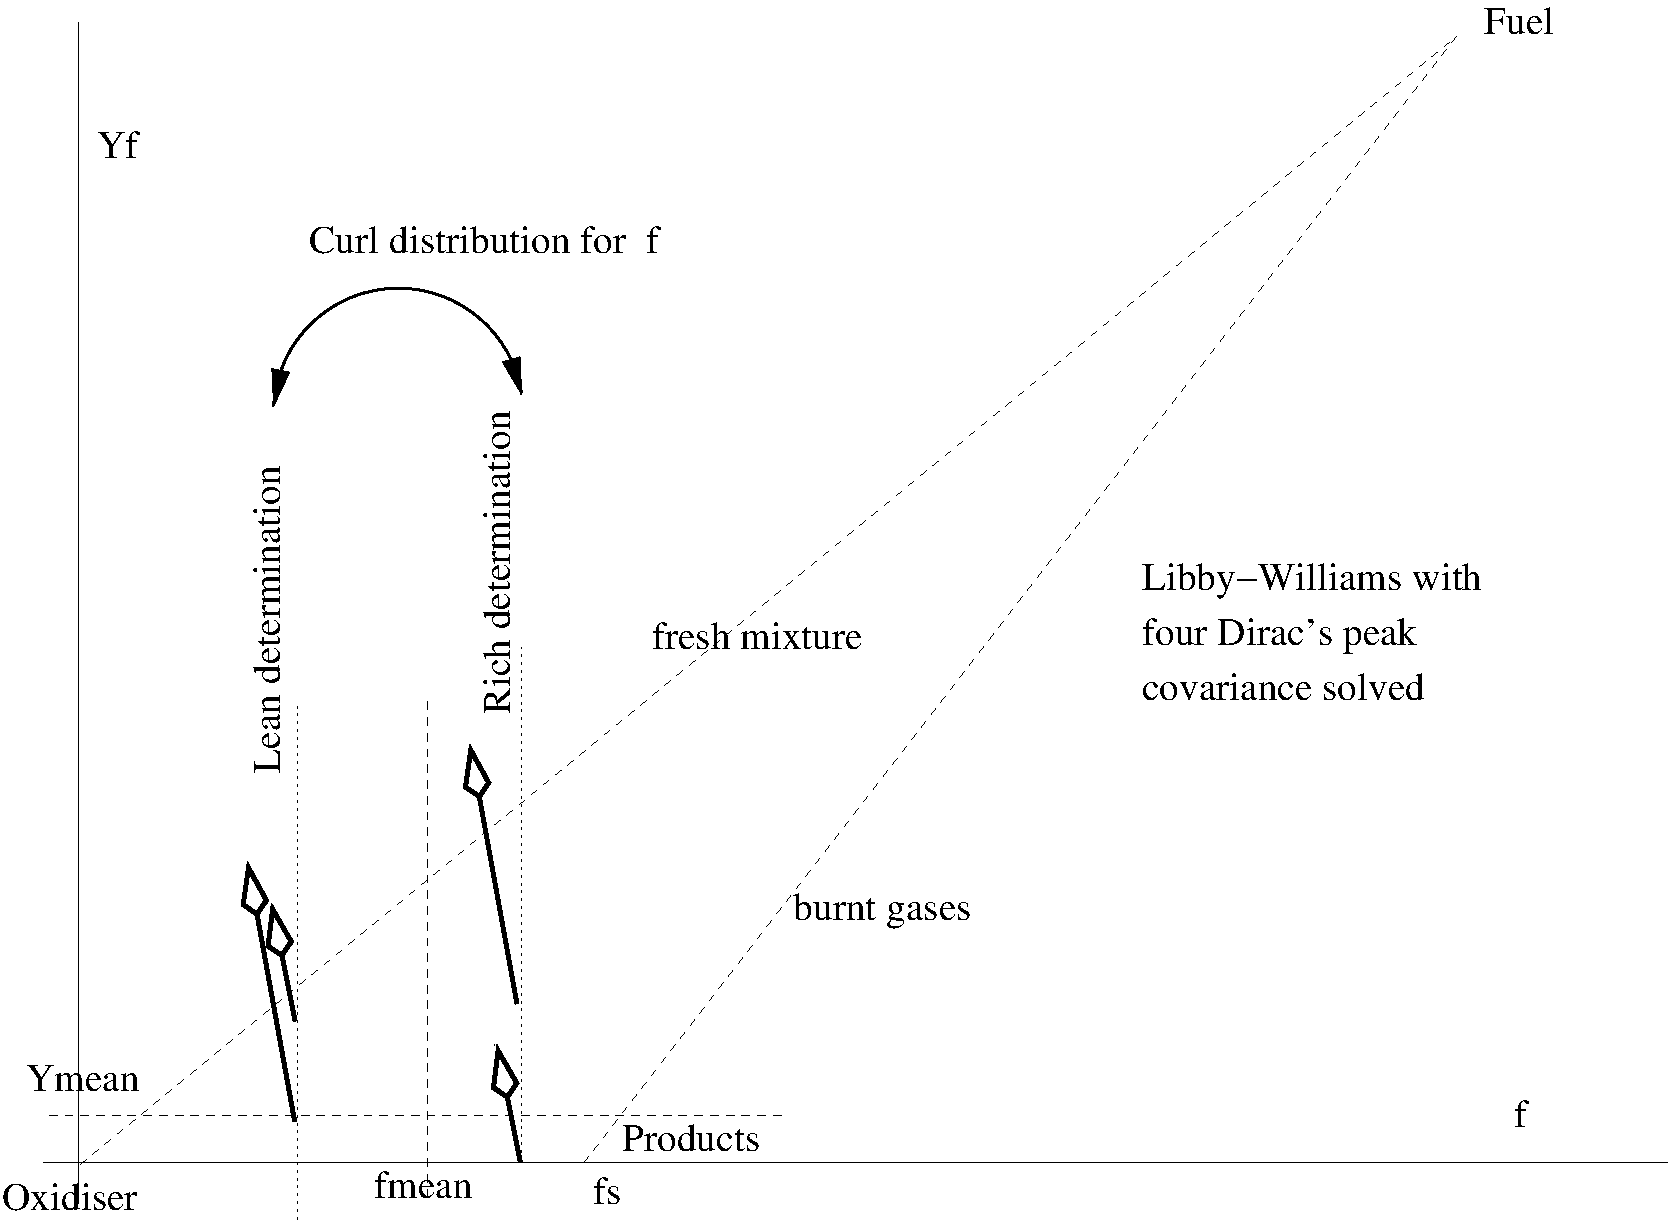
\includegraphics[width=0.8\textwidth]{LW4}}
\caption{PDF form in LWP approach: succesive modified Curl distributions.}
\end{figure}
%========================================

In adiabatic conditions, the temperature can be computed for every pair $(f,Yfuel)$, allowing the determination of the kinetic constant.

As previously, with heat losses, it is assumed that the hottest gases have lost
the more (of their thermal enthalpy), the enthalpy of the products at
stoechiometric point $(fs,0)$ is an auxiliary variable, the enthaply being
considered as a piecewise bilinear function. Fitting mean transported enthalpy
and integrated ones, allows to determine the enthalpy of stoechiometric
products, then the enthalpy and temperature in the peaks conditions and, \emph{in fine} the reactions fluxes.

%=====================================
\subsection{Numerical Recipies for PDF}
%=====================================

Some applied mathematics are involved in pdf parameters determination (rectangle
and modified Curl) and for integration (species
mass fraction, temperature, density and so on).

Some tests, done by \cite{Sapa:2011} show weak discrepancies between species mass
fraction with respect to the shape of the PDF (among Beta, rectangle and peaks,
Curl; for similar mean during variance dissipation).

%======================================================================
\subsubsection{Rectangle and Dirac's peaks probability density function}
%======================================================================

This type of pdf is used in diffusion flames both for gas combustion or
dispersed fuel ones (coal and heavy fuel oil). In gas mixture, the pdf is build
for an equivalence ratio for fuel (inert scalar variable) ranging on [0, 1]. For
dispersed fuel, due to vaporisation, or pyrolysis, and heterogeneous combustion
two or three gaseous fuels are taken in account, each of them having its own
inert scalar, so the PDF is build for an inert scalar which is the total of
passive scalars for volatiles matter (coal and biomass) or hydrocarbon vapor
(heavy
fuel oil). The algorithm for pdf parameters determination, can be written in a general form on every variable's range.

If the allowed range for the variable is [$f_{\min} ; f_{\max}$], knowing the
mean and variance of the variable allow to determine first the shape (alone
rectangle, rectangle and one Dirac's peak at one boundary, two Dirac's peak at
boundaries and rectangle) and then, the three pertinent parameters (three
conditions given by momenta $m_{0}=1, m_{1}=\text{mean},
m_{2}=\text{mean}^{2}+\text{variance}$).

%==================
\begin{enumerate}
\item For a lonesome rectangle Dirac's peak intensity is null, the three
  parameters are: the begining and end values of the rectangle and its heigth.
\item For a rectangle with a Dirac's peak at one boundary (which is determined
  during the choice of shape), one of the rectangle edge is fixed at this
  boundary, so the three parameters are : the other rectangle edge, height of
  rectangle, intensity of the Dirac's peak.
\item For a two Dirac's peak distribution, both rectangle edges are at the
  boudaries, so the parameters are the rectangle height and the Dirac's peak
  intensity.
\end{enumerate}
%==================

The choice between the four possible forms can be done by previous test on the
variance. Defining $v_1$ and $v_2$ by:
\begin{eqnarray}
%---------------
\overline{f} \le \frac{1}{2} &\Rightarrow& v1 = \frac{\overline{f}^2}{3} \quad ; \quad v2 = \frac{\overline{f}.(2-3.\overline{f})}{3}                   \\
\overline{f} \ge \frac{1}{2} &\Rightarrow& v1 = \frac{(1-\overline{f})^2}{3} \quad ; \quad v2 = \frac{(1-\overline{f}).(2-3.(1-\overline{f}))}{3}       \\
\forall \overline{f} &\Rightarrow& v1= \min\left( \frac{\overline{f}^2}{3} ; \frac{(1-\overline{f})^2}{3}\right)                                        \\
\forall \overline{f} &\Rightarrow& v2= \max\left( \frac{\overline{f}.(2-3.\overline{f})}{3} ; \frac{(1-\overline{f}).(2-3.(1-\overline{f}))}{3}\right)
\end{eqnarray}
Depending on the value of variance and naming $D_0$ and $D_1$, the Dirac's peak
magnitude, $f_2$ and $f_3$ the begining and end of the rectangle and h its
height, the determination is:

\begin{enumerate}
\item if the variance is lower than $v_1$, the pdf is only made of a rectangle (symetrical with respect to the mean)
\begin{equation}
%---------------
D_0 = D_1 = 0 ~;~ f_2 = \tilde{f} - \sqrt{3\widetilde{f^{''2}}} ~;~ f_2 = \tilde{f} - \sqrt{3\widetilde{f^{''2}}}
%---------------
\end{equation}
\item if the variance is greater than $v_2$, the pdf is made of two Dirac's peak
  and a rectangle (over all range); (be careful the mean of square is neither
  the variance nor the square of mean; but the sum of them)
\begin{equation}
%---------------
f_2 = 0 ~;~ f_3 = 1 ~;~ D_0 = 3.\widetilde{f^2}-4.\tilde{f}+1 ~;~ D_1 = 3.\widetilde{f^2}-2.\tilde{f}
%---------------
\end{equation}
\item if the variance is greater than $v_1$ and lower than $v_2$, the pdf is
  made of only one Dirac's peak (in 0 if the mean is lower than one half in 1
  otherwise) and a rectangle.
\begin{eqnarray}
%---------------
\tilde{f} \le \frac{1}{2} & \Rightarrow & D_1 = 0 ~;~ f_2 = 0 ~;~ f_3 = \frac{3.\widetilde{f^2}}{2.\tilde{f}} ~;~ D_0 = 1-2. \left(\frac{\tilde{f}}{f_3} \right)  \\
\tilde{f} \ge \frac{1}{2} & \Rightarrow & D_0 = 0 ~;~ f_3 = 1 ~;~ f_2 = \frac{3.\widetilde{f^2}-4.\tilde{f}+1}{2.(\tilde{f}-1)} ~;~ D_1 = \frac{2.\tilde{f}-1-f_2}{1-f_2} \nonumber
\end{eqnarray}
\item every time, the height of the rectangle obeys the same relation :
\begin{equation}
h = \frac{1-D_0-D_1}{f_3-f_2}
\end{equation}
\end{enumerate}
%==================

%================================
\subsubsection{Curl distribution}
%================================

The Curl distribution is only composed of two Dirac's peaks. Such a distribution
needs four parameters (two positions and two amplitudes), only two moments (mean
and variance) are known, the completness is the third, so an extra assumption is
needed : the standard Curl distribution assumed amplitudes values (the mean for
the richer, the remainder to one for the leaner), a modification of the Curl
distribution is given by an extra constraint : use of recurrence relation
between Beta function allows to determine the third moment ( linked with
skewness) and to modify amplitudes of peaks. In this \CS~ release, only
regular Curl distribution is implemented and used (discrepancies in species mass
fractions using the modified Curl are not worthy of this option introduction).
Looking for $P_1$ and $P_2$ the amplitudes, and $f_1$ and $f_2$ the positions,
with constraints from completeness, mean and variance, it comes :

\begin{eqnarray}
%---------------
\label{eq:P1P2}
        P_1 + P_2 & = & 1 \Rightarrow P_2 = 1-P_1                                    \label{Eqs_xx1} \\
  P_1.f_1 + P_2.f_2 & = & \tilde{f}  \Rightarrow f2 = \frac{\tilde{f}-P_1.f1}{1-P_1}   \label{Eqs_xx2} \\
P_1.f_1^2+P_2.f_2^2 & = & \widetilde{f^2} = \tilde{f}^2+\widetilde{f{''}^2} \Rightarrow \label{Eqs_xx3} \\
                &   & f_1 = \tilde{f} - \sqrt{\widetilde{f{''}^2} . \frac{1-P_1}{P_1}} \label{Eqs_xx4} \\
                &   & f_2 = \tilde{f} + \sqrt{\widetilde{f{''}^2} . \frac{P_1}{1-P_1}} \label{Eqs_xx5}
%---------------
\end{eqnarray}
$f_1$ and $f_2$ may be inside [0, 1], the first proposal by Curl (in the context
of liquid-liquid extraction, the interfacial mass flux does not modify mass of
each phases) is:
\begin{eqnarray}
%---------------
&& P_1 = 1-\tilde{f} ; P_2=\tilde{f}                                                  \nonumber \\
&& f_1 = \tilde{f}.\left\{~ 1-\sqrt{\frac{\widetilde{f"^2}}{\tilde{f}.(1-\tilde{f})}} ~\right\} \label{Eqs_xx6}
%---------------
\end{eqnarray}
Obviously, maximal value of variance induces Dirac's peak positionned at boundaries.

Formulae in \eqref{eq:P1P2} can be used to determine the peak's magnitude if any
extra condition is retained. In the context of pdf, the Beta function have the
fame of fairly good representation of micro-mixing, so the third momentum of a
Beta distribution is easy to determine (thanks to recurrency), used as a
constraint for a modified Curl model, it comes :
\begin{eqnarray}
&&\widetilde{f^3}     = \frac{\alpha +2}{\alpha+\beta+2} .\widetilde{f^2}  \label{Eqs_xx7}\\
&&\widetilde{f{''}^3} =2 . \widetilde{f{''}^2}^2 . \frac{1-2.\tilde{f}}{\tilde{f}.(1-\tilde{f})+\widetilde{f{''}^2}}  \label{Eqs_xx8}\\
&&P_1^2~\left\{~          4+\frac{\widetilde{f{''}^3}^2}{\widetilde{f{''}^2}^3}~\right\}
                 -P_1~\left\{~ 4+\frac{\widetilde{f{''}^3}^2}{\widetilde{f{''}^2}^3}~\right\}+1=0 \label{Eqs_xx9}
\end{eqnarray}
Some numerical evaluations don't show large discrepancies ({\small among mass fraction or temperature}) so this option is not currently available.

\newpage
%===============================

